Ogni componente ha deciso che si impegnerà al massimo delle ore, ovvero 100: quindi in totale si otterranno 700 ore. Il preventivo è stato calcolato sulla base del costo orario per ruolo presente nel Regolamento del Progetto Didattico. La suddivisione dei ruoli per persona è stata fatta nel modo più equo possibile,in modo da dare a tutti i membri la possibilità di 
sperimentare ogni ruolo. \\ 
All'interno delle tabelle sono state utilizzate tali abbreviazioni per consentire una lettura più scorrevole:
\begin{itemize}
    \item \textbf{Re}: Responsabile;
    \item \textbf{Am}: Amministratore;
    \item \textbf{An}: Analista;
    \item \textbf{Pt}: Progettista;
    \item \textbf{Pr}: Programmatore;
    \item \textbf{Ve}: Verificatore.
\end{itemize}

\subsection{Primo incremento} 
{
    \subsubsection{Prospetto orario}
    {
    Il gruppo per il primo incremento si impegna a rispettare la suddivisione oraria dei ruoli come riportato in tabella:
      \setlength{\freewidth}{\dimexpr\textwidth-30\tabcolsep}
      \renewcommand{\arraystretch}{1.0}
      \setlength{\aboverulesep}{0pt}
      \setlength{\belowrulesep}{0pt}
      \rowcolors{2}{Arancione!10}{white}
      \begin{longtable}{C{.4\freewidth} C{.1\freewidth} C{.1\freewidth} C{.1\freewidth} C{.1\freewidth} C{.1\freewidth} C{.1\freewidth} C{.1\freewidth} C{.1\freewidth}}
      \toprule
      \rowcolor{Arancione}
      \textcolor{white}{\textbf{Componente}}&
      \textcolor{white}{\textbf{Re}}&
      \textcolor{white}{\textbf{Am}}&
      \textcolor{white}{\textbf{An}}&
      \textcolor{white}{\textbf{Pt}}&
      \textcolor{white}{\textbf{Pr}}&
      \textcolor{white}{\textbf{Ve}}&
      \textcolor{white}{\textbf{Ore}}\\
      \toprule
      \endhead

      Arena Angela & - & 4 & - & - & - & 5 & 9 \\
      Bellò Marco & 2 & 4 & - & - & - & 1 & 7 \\
      Bousapnamene & - & 3 & - & - & - & 4 & 7 \\
      Di Fant Tommaso & - & 4 & - & - & - & 4 & 8 \\
      Tossuto Matteo & - & 5 & - & - & - & 4 & 9 \\
      Volpato Marco & 3 & 2 & - & - & - & 2 & 7 \\
      Zanatta Giulio & - & 5 & - & - & - & 4 & 9 \\
      Totali & 5 & 27 & - & - & - & 24 & 56 \\
      \bottomrule
      \rowcolor{white}
      \\
      \caption{Primo incremento - Suddivisone ore per ruolo}
      \end{longtable} 

      \begin{figure}[H]
        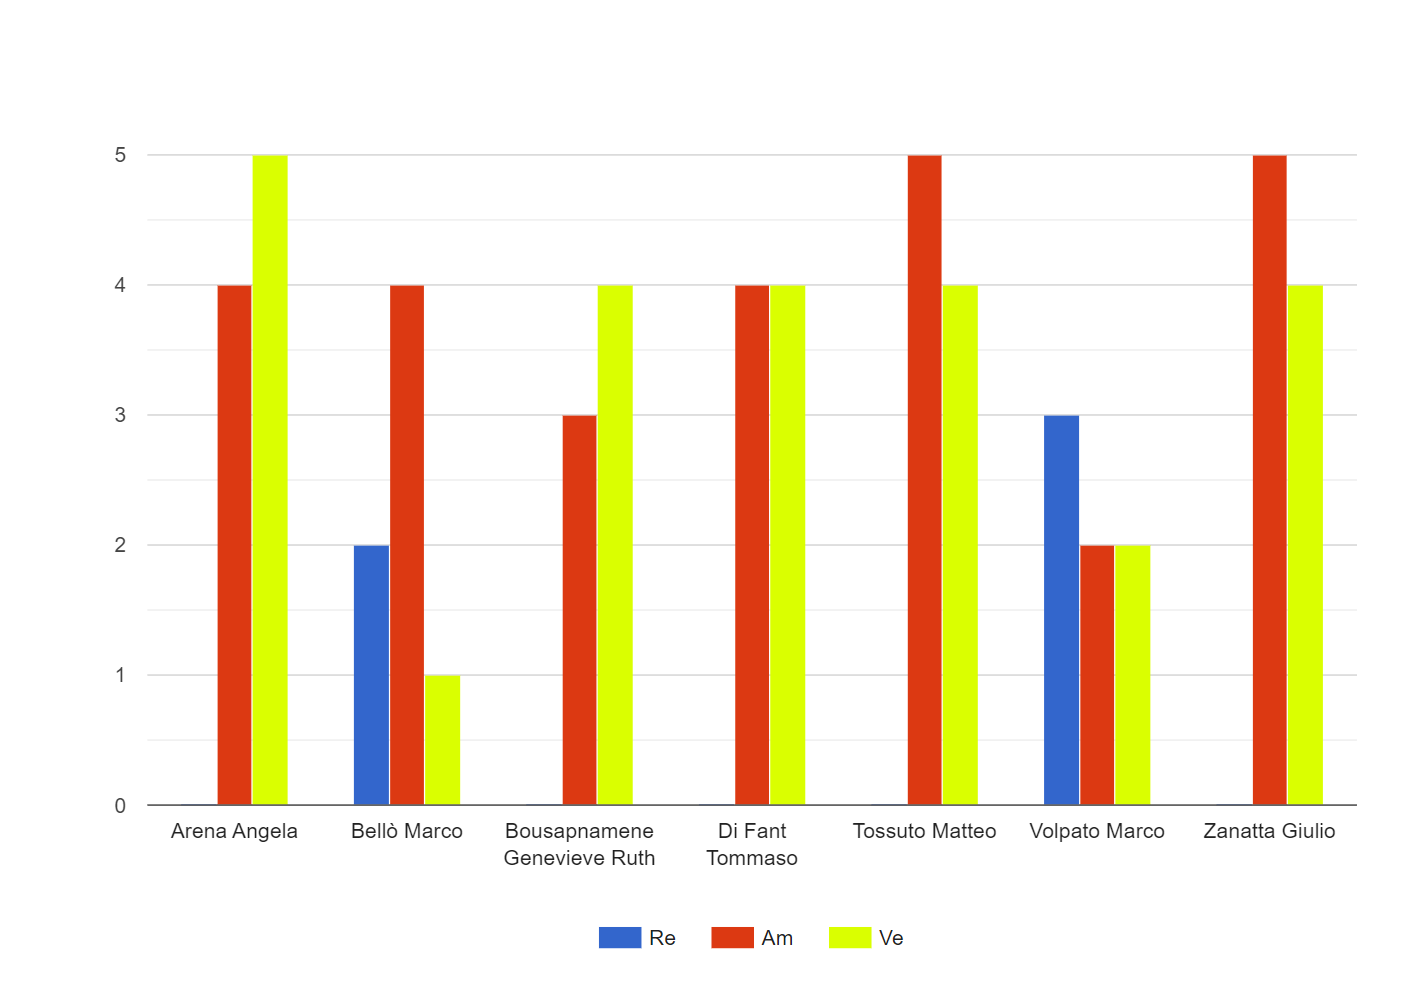
\includegraphics[width=15cm]{sezioni/images/primo.png}
        \centering
        \\
        \caption{Primo incremento - Istogramma suddivisione ore per ruolo}
     \end{figure}
    }

    \subsubsection{Prospetto Economico}
    {
        \setlength{\freewidth}{\dimexpr\textwidth-30\tabcolsep}
        \renewcommand{\arraystretch}{1.0}
        \setlength{\aboverulesep}{0pt}
        \setlength{\belowrulesep}{0pt}
        \rowcolors{2}{Arancione!10}{white}
        \begin{longtable}{C{.3\freewidth} C{.2\freewidth} C{.2\freewidth}}
          \toprule
        \rowcolor{Arancione}
        \textcolor{white}{\textbf{Ruolo}}&
        \textcolor{white}{\textbf{Ore}}&
        \textcolor{white}{\textbf{Costo}}\\
        \toprule
        \endhead
            
        Responsabile & 5 & \euro150\\        
        Amministratore & 27 & \euro540\\        
        Analista & - &-\\        
        Progettista&-&-\\        
        Programmatore&-&-\\
        Verificatore&24 & \euro360\\
        Totale&56&\euro1050\\
        \bottomrule
        \\
        \rowcolor{white}
        \caption{Primo incremento - Costo per ruolo}

        \end{longtable}
        \begin{figure}[H]
          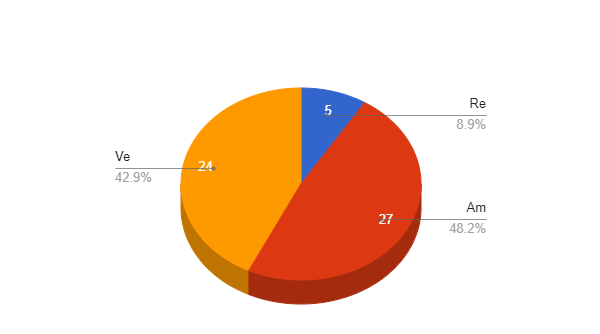
\includegraphics[width=15cm]{sezioni/images/primoT.png}
          \centering
          \caption{Primo incremento - Grafico a torta costo per ruolo}
       \end{figure}
    }
}
  
  \subsection{Secondo incremento} 
    {
    \subsubsection{Prospetto orario}
    {
    Il gruppo per il secondo incremento si impegna a rispettare la suddivisione oraria dei ruoli come riportato in tabella:
      \setlength{\freewidth}{\dimexpr\textwidth-30\tabcolsep}
      \renewcommand{\arraystretch}{1.0}
      \setlength{\aboverulesep}{0pt}
      \setlength{\belowrulesep}{0pt}
      \rowcolors{2}{Arancione!10}{white}
      \begin{longtable}{C{.4\freewidth} C{.1\freewidth} C{.1\freewidth} C{.1\freewidth} C{.1\freewidth} C{.1\freewidth} C{.1\freewidth} C{.1\freewidth} C{.1\freewidth}}
      \toprule
      \rowcolor{Arancione}
      \textcolor{white}{\textbf{Componente}}&
      \textcolor{white}{\textbf{Re}}&
      \textcolor{white}{\textbf{Am}}&
      \textcolor{white}{\textbf{An}}&
      \textcolor{white}{\textbf{Pt}}&
      \textcolor{white}{\textbf{Pr}}&
      \textcolor{white}{\textbf{Ve}}&
      \textcolor{white}{\textbf{Ore}}\\
      \toprule
      \endhead

      Arena Angela & - & - & 7  & - & - & 4 & 11 \\      
      Bellò Marco & - & - & 8 & - & - & 4 & 12 \\      
      Bousapnamene & 5 & - & 2 & - & - & 4 & 11 \\      
      Di Fant Tommaso & - & - & 6 & - & - & 4 & 10 \\      
      Tossuto Matteo & - & - & 9 & - & - & 1 & 10 \\      
      Volpato Marco & - & - & 9 & - & - & 2 & 11 \\      
      Zanatta Giulio & - & - & 8 & - & - & 4 & 12 \\      
      Totali & 5 & - & 49 & - & - & 23 & 77 \\
      \bottomrule
      \rowcolor{white}
      \\
      \caption{\centering{Secondo incremento - Suddivisone ore per ruolo}}

      \end{longtable} 
      \begin{figure}[H]
        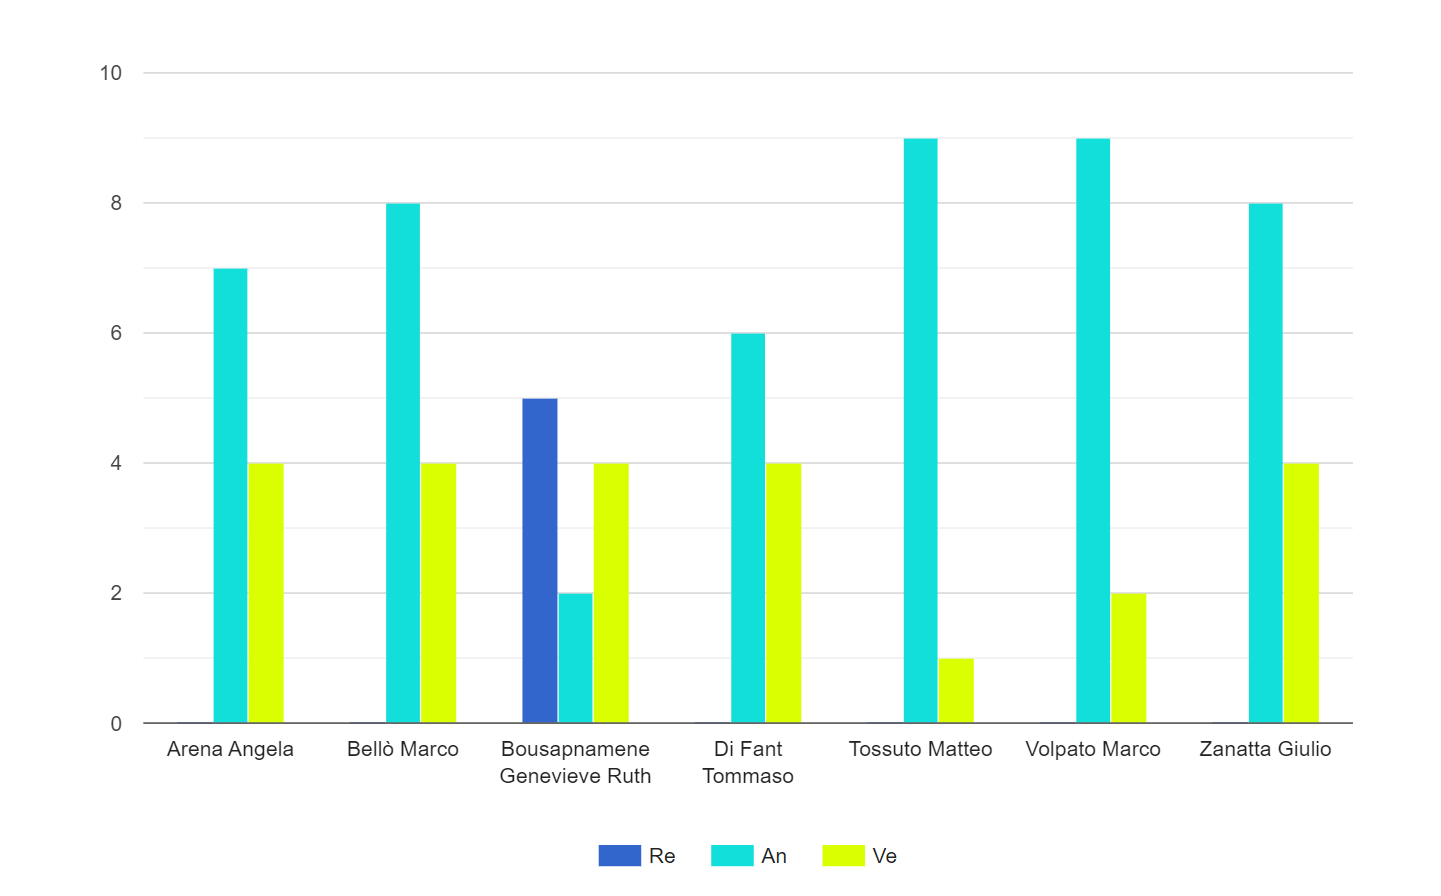
\includegraphics[width=15cm]{sezioni/images/secondo.png}
        \centering
        \caption{Secondo incremento - Istogramma suddivisione ore per ruolo}
     \end{figure}
      
    }
    

    \subsubsection{Prospetto Economico}
    {
        \setlength{\freewidth}{\dimexpr\textwidth-30\tabcolsep}
        \renewcommand{\arraystretch}{1.0}
        \setlength{\aboverulesep}{0pt}
        \setlength{\belowrulesep}{0pt}
        \rowcolors{2}{Arancione!10}{white}
        \begin{longtable}{C{.4\freewidth} C{.2\freewidth} C{.2\freewidth} C{.2\freewidth} C{.2\freewidth} C{.2\freewidth} C{.2\freewidth} C{.2\freewidth} C{.2\freewidth}}
          \toprule
        \rowcolor{Arancione}
        \textcolor{white}{\textbf{Ruolo}}&
        \textcolor{white}{\textbf{Ore}}&
        \textcolor{white}{\textbf{Costo}}\\
        \toprule
        \endhead
            
        Responsabile  & 5 & \euro150\\        
        Amministratore  & -&  \\        
        Analista &49 & \euro1225\\        
        Progettista &- &\\        
        Programmatore &- & \\        
        Verificatore &23 &\euro345\\        
        Totale&77&\euro1720\\
        \bottomrule
      	\\
      	\rowcolor{white}
        \caption{Secondo incremento - Costo per ruolo}

        \end{longtable}
        \begin{figure}[H]
          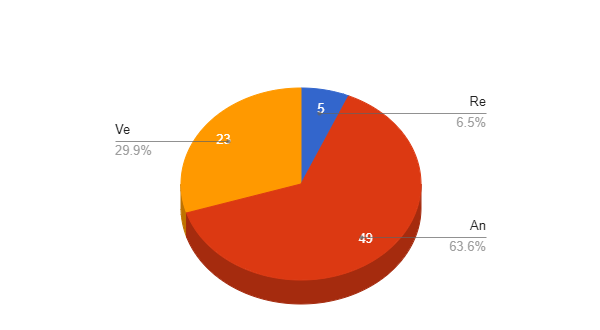
\includegraphics[width=15cm]{sezioni/images/secondoT.png}
          \centering
          \caption{Secondo incremento - Grafico a torta costo per ruolo}
       \end{figure}
    }
    }

    \subsection{Terzo incremento} 
    {
    \subsubsection{Prospetto orario}
    {
    Il gruppo per il terzo incremento si impegna a rispettare la suddivisione oraria dei ruoli come riportato in tabella:
      \setlength{\freewidth}{\dimexpr\textwidth-30\tabcolsep}
      \renewcommand{\arraystretch}{1.0}
      \setlength{\aboverulesep}{0pt}
      \setlength{\belowrulesep}{0pt}
      \rowcolors{2}{Arancione!10}{white}
      \begin{longtable}{C{.4\freewidth} C{.1\freewidth} C{.1\freewidth} C{.1\freewidth} C{.1\freewidth} C{.1\freewidth} C{.1\freewidth} C{.1\freewidth} C{.1\freewidth}}
      \toprule
      \rowcolor{Arancione}
      \textcolor{white}{\textbf{Componente}}&
      \textcolor{white}{\textbf{Re}}&
      \textcolor{white}{\textbf{Am}}&
      \textcolor{white}{\textbf{An}}&
      \textcolor{white}{\textbf{Pt}}&
      \textcolor{white}{\textbf{Pr}}&
      \textcolor{white}{\textbf{Ve}}&
      \textcolor{white}{\textbf{Ore}}\\
      \toprule
      \endhead

      Arena Angela & 2 & - & 4  & 2 & 2 & 4 & 14 \\      
      Bellò Marco & - & 1 & 1 & 5 & 7 & - & 14 \\      
      Bousapnamene & - & 2 & - & 6 & 4 & 2 & 14 \\      
      Di Fant Tommaso & - & - & - & 7 & 8 & 1 & 16 \\      
      Tossuto Matteo & - & - & 4 & 3 & 7 & - & 14 \\      
      Volpato Marco & - & - & - & 3 & 9 & 2 & 14 \\      
      Zanatta Giulio & 3 & 2 & - & - & 5 & 3 & 13 \\      
      Totali & 5 & 5 & 9 & 26 & 42 & 12 & 99 \\
      \bottomrule
      \rowcolor{white}
      \\
      \caption{Terzo incremento - Suddivisone ore per ruolo}

      \end{longtable} 

      \begin{figure}[H]
        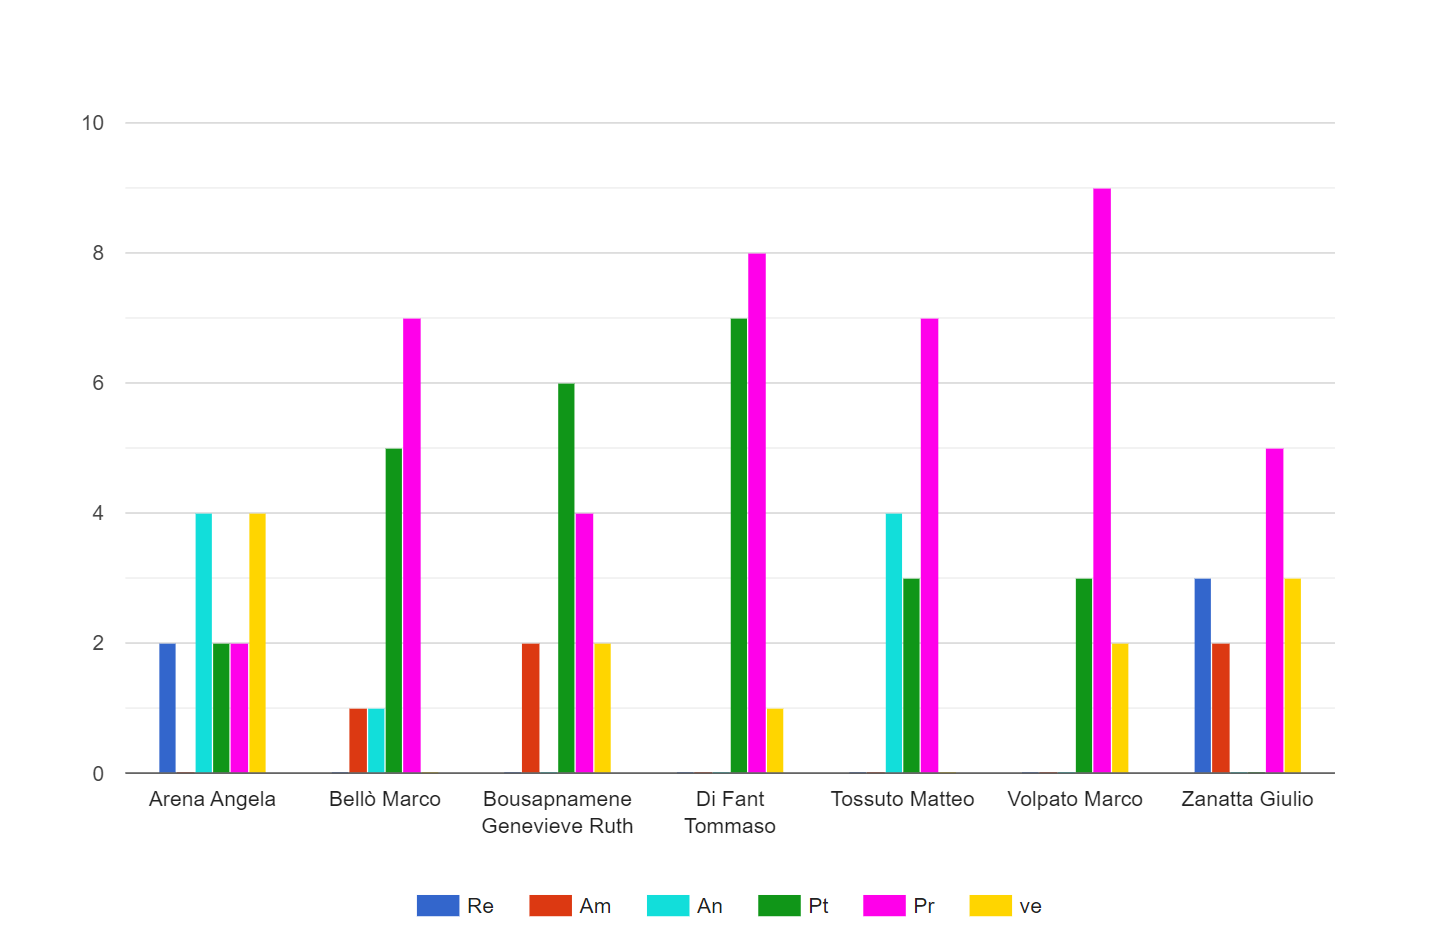
\includegraphics[width=15cm]{sezioni/images/terzo.png}
        \centering
        \caption{Terzo incremento - Istogramma suddivisione ore per ruolo}
     \end{figure}
    }

    \subsubsection{Prospetto Economico}
    {
        \setlength{\freewidth}{\dimexpr\textwidth-30\tabcolsep}
        \renewcommand{\arraystretch}{1.0}
        \setlength{\aboverulesep}{0pt}
        \setlength{\belowrulesep}{0pt}
        \rowcolors{2}{Arancione!10}{white}
        \begin{longtable}{C{.4\freewidth} C{.2\freewidth} C{.2\freewidth} C{.2\freewidth} C{.2\freewidth} C{.2\freewidth} C{.2\freewidth} C{.2\freewidth} C{.2\freewidth}}
          \toprule
        \rowcolor{Arancione}
        \textcolor{white}{\textbf{Ruolo}}&
        \textcolor{white}{\textbf{Ore}}&
        \textcolor{white}{\textbf{Costo}}\\
        \toprule
        \endhead
            
        Responsabile  & 5 & \euro150\\
        Amministratore  & 5 & \euro100 \\
        Analista &9 & \euro225\\
        Progettista &26 & \euro650\\
        Programmatore &42 & \euro630\\
        Verificatore &12 & \euro180\\
        Totale&99&\euro1935\\
        \bottomrule
      \\
      \rowcolor{white}
        \caption{Terzo incremento - Costo per ruolo}

        \end{longtable}
        \begin{figure}[H]
          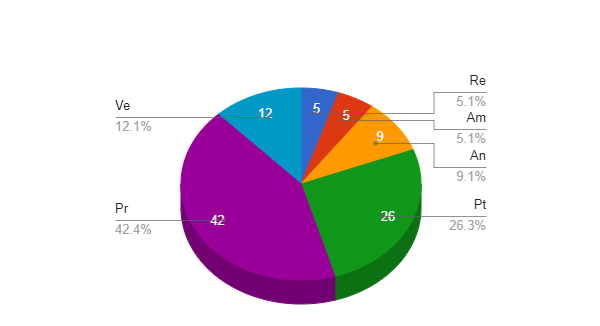
\includegraphics[width=15cm]{sezioni/images/terzoT.png}
          \centering
          \caption{Terzo incremento - Grafico a torta costo per ruolo}
       \end{figure}
    }
    }

    \subsection{Quarto incremento} 
    {
    \subsubsection{Prospetto orario}
    {
    Il gruppo per il quarto incremento si impegna a rispettare la suddivisione oraria dei ruoli come riportato in tabella:
      \setlength{\freewidth}{\dimexpr\textwidth-30\tabcolsep}
      \renewcommand{\arraystretch}{1.0}
      \setlength{\aboverulesep}{0pt}
      \setlength{\belowrulesep}{0pt}
      \rowcolors{2}{Arancione!10}{white}
      \begin{longtable}{C{.4\freewidth} C{.1\freewidth} C{.1\freewidth} C{.1\freewidth} C{.1\freewidth} C{.1\freewidth} C{.1\freewidth} C{.1\freewidth} C{.1\freewidth}}
      \toprule
      \rowcolor{Arancione}
      \textcolor{white}{\textbf{Componente}}&
      \textcolor{white}{\textbf{Re}}&
      \textcolor{white}{\textbf{Am}}&
      \textcolor{white}{\textbf{An}}&
      \textcolor{white}{\textbf{Pt}}&
      \textcolor{white}{\textbf{Pr}}&
      \textcolor{white}{\textbf{Ve}}&
      \textcolor{white}{\textbf{Ore}}\\
      \toprule
      \endhead

      Arena Angela & - & 2 & -  & 10 & - & 2 & 14 \\      
      Bellò Marco & - & 2 & - & 9 & - & 2 & 13 \\      
      Bousapnamene & - & 1 & - & 10 & - & 2 & 13 \\      
      Di Fant Tommaso & 3 & - & - & 8 & - & 4 & 13 \\      
      Tossuto Matteo & 2 & - & - & 8 & - & 3 & 15 \\      
      Volpato Marco & - & 1 & - & 12 & - & 2 & 16 \\      
      Zanatta Giulio & - & 1 & - & 11 & - & 3 & 15 \\      
      Totali & 5 & 7 & - & 68 & - & 18 & 101 \\
      \bottomrule
      \rowcolor{white}
      \\
      \caption{\centering{Quarto incremento - Suddivisione ore per ruolo}}

      \end{longtable} 

      \begin{figure}[H]
        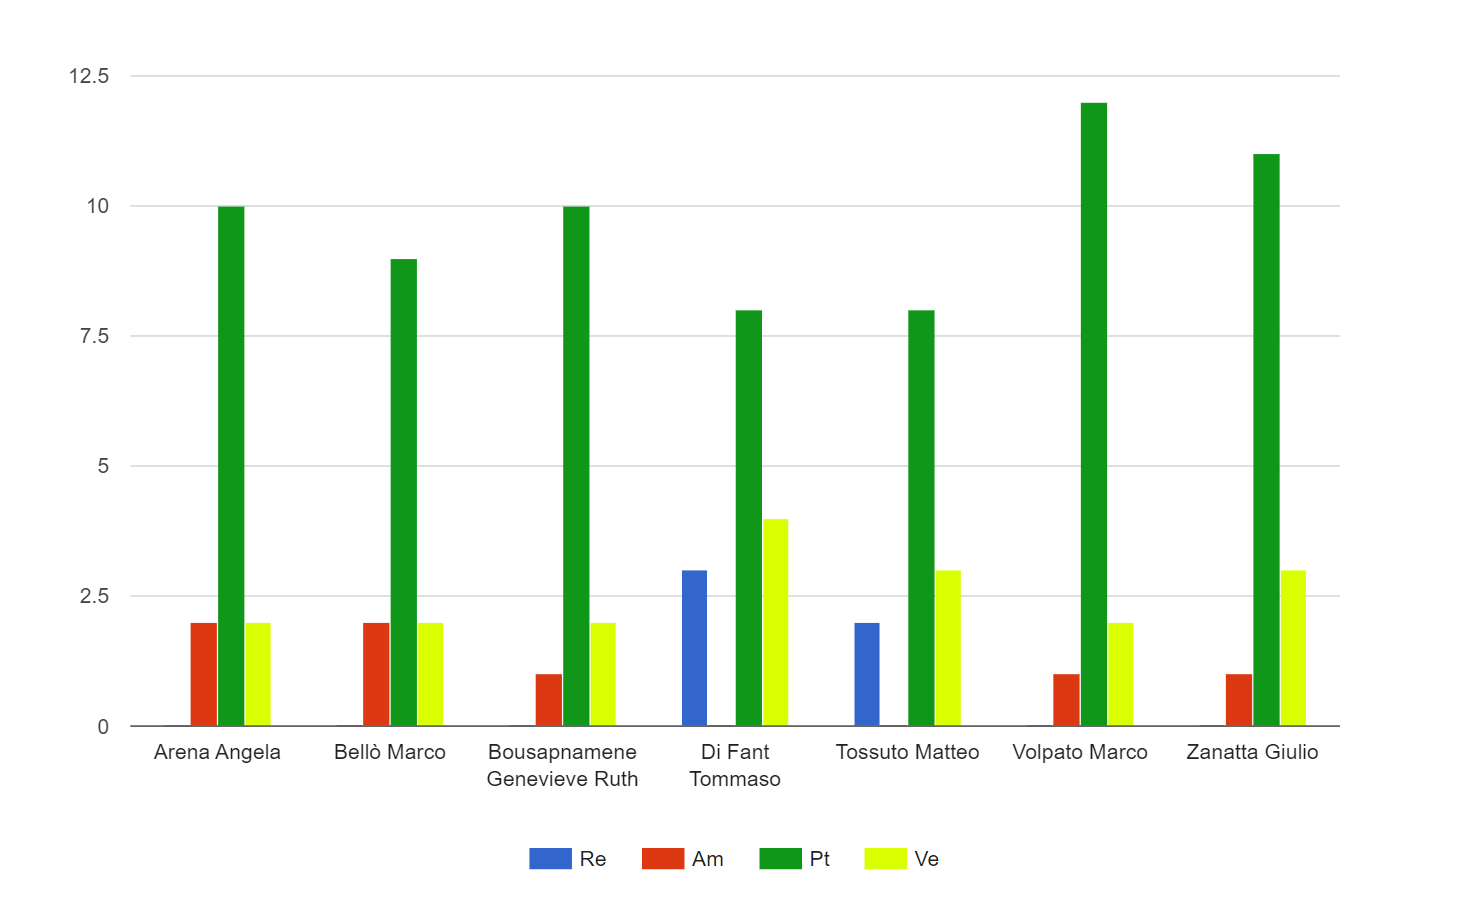
\includegraphics[width=15cm]{sezioni/images/quarto.png}
        \centering
        \caption{Quarto incremento - Istogramma suddivisione ore per ruolo}
     \end{figure}
    }

    \subsubsection{Prospetto Economico}
    {
        \setlength{\freewidth}{\dimexpr\textwidth-30\tabcolsep}
        \renewcommand{\arraystretch}{1.0}
        \setlength{\aboverulesep}{0pt}
        \setlength{\belowrulesep}{0pt}
        \rowcolors{2}{Arancione!10}{white}
        \begin{longtable}{C{.4\freewidth} C{.2\freewidth} C{.2\freewidth} C{.2\freewidth} C{.2\freewidth} C{.2\freewidth} C{.2\freewidth} C{.2\freewidth} C{.2\freewidth}}
          \toprule
        \rowcolor{Arancione}
        \textcolor{white}{\textbf{Ruolo}}&
        \textcolor{white}{\textbf{Ore}}&
        \textcolor{white}{\textbf{Costo}}\\
        \toprule
        \endhead
            
        Responsabile  & 5 & \euro150\\
        Amministratore  & 7& \euro140 \\
        Analista &- & -\\
        Progettista &68 &\euro1700\\
        Programmatore &- & -\\
        Verificatore &18 &\euro270\\
        Totale&101&\euro2260\\
        \bottomrule
      \\
      \rowcolor{white}
        \caption{Quarto incremento - Costo per ruolo}

        \end{longtable}
        \begin{figure}[H]
          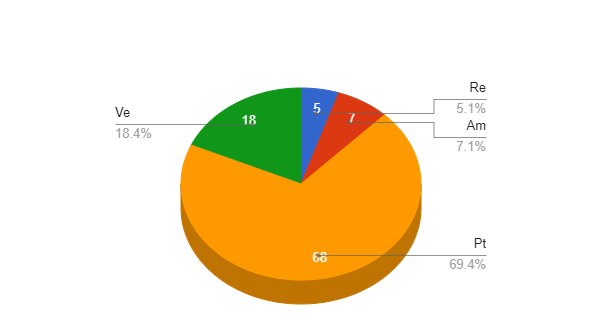
\includegraphics[width=15cm]{sezioni/images/quartoT.png}
          \centering
          \caption{Quarto incremento - Grafico a torta costo per ruolo}
       \end{figure}
    }
    }

    \subsection{Quinto incremento} 
    {
    \subsubsection{Prospetto orario}
    {
    Il gruppo per il quinto incremento si impegna a rispettare la suddivisione oraria dei ruoli come riportato in tabella:
      \setlength{\freewidth}{\dimexpr\textwidth-30\tabcolsep}
      \renewcommand{\arraystretch}{1.0}
      \setlength{\aboverulesep}{0pt}
      \setlength{\belowrulesep}{0pt}
      \rowcolors{2}{Arancione!10}{white}
      \begin{longtable}{C{.4\freewidth} C{.1\freewidth} C{.1\freewidth} C{.1\freewidth} C{.1\freewidth} C{.1\freewidth} C{.1\freewidth} C{.1\freewidth} C{.1\freewidth}}
      \toprule
      \rowcolor{Arancione}
      \textcolor{white}{\textbf{Componente}}&
      \textcolor{white}{\textbf{Re}}&
      \textcolor{white}{\textbf{Am}}&
      \textcolor{white}{\textbf{An}}&
      \textcolor{white}{\textbf{Pt}}&
      \textcolor{white}{\textbf{Pr}}&
      \textcolor{white}{\textbf{Ve}}&
      \textcolor{white}{\textbf{Ore}}\\
      \toprule
      \endhead

      Arena Angela & - & 3 & -  & 6 & 10 & 2 & 21 \\      
      Bellò Marco & - & - & - & 6 & 10 & 3 & 19 \\      
      Bousapnamene & 2 & - & - & 5 & 10 & 4 & 21 \\      
      Di Fant Tommaso & - & 1 & - & 6 & 12 & 3 & 22 \\      
      Tossuto Matteo & - & 1 & - & 8 & 12 & 1 & 22 \\      
      Volpato Marco & 3 & - & - & 4 & 10 & 5 & 22 \\      
      Zanatta Giulio & - & 2 & - & 6 & 11 & 3 & 21 \\      
      Totali & 5 & 7 & - & 41 & 75 & 21 & 148 \\
      \bottomrule
      \rowcolor{white}
      \\
      \caption{\centering{Quinto incremento - Suddivisione ore per ruolo}}
      \end{longtable} 

      \begin{figure}[H]
        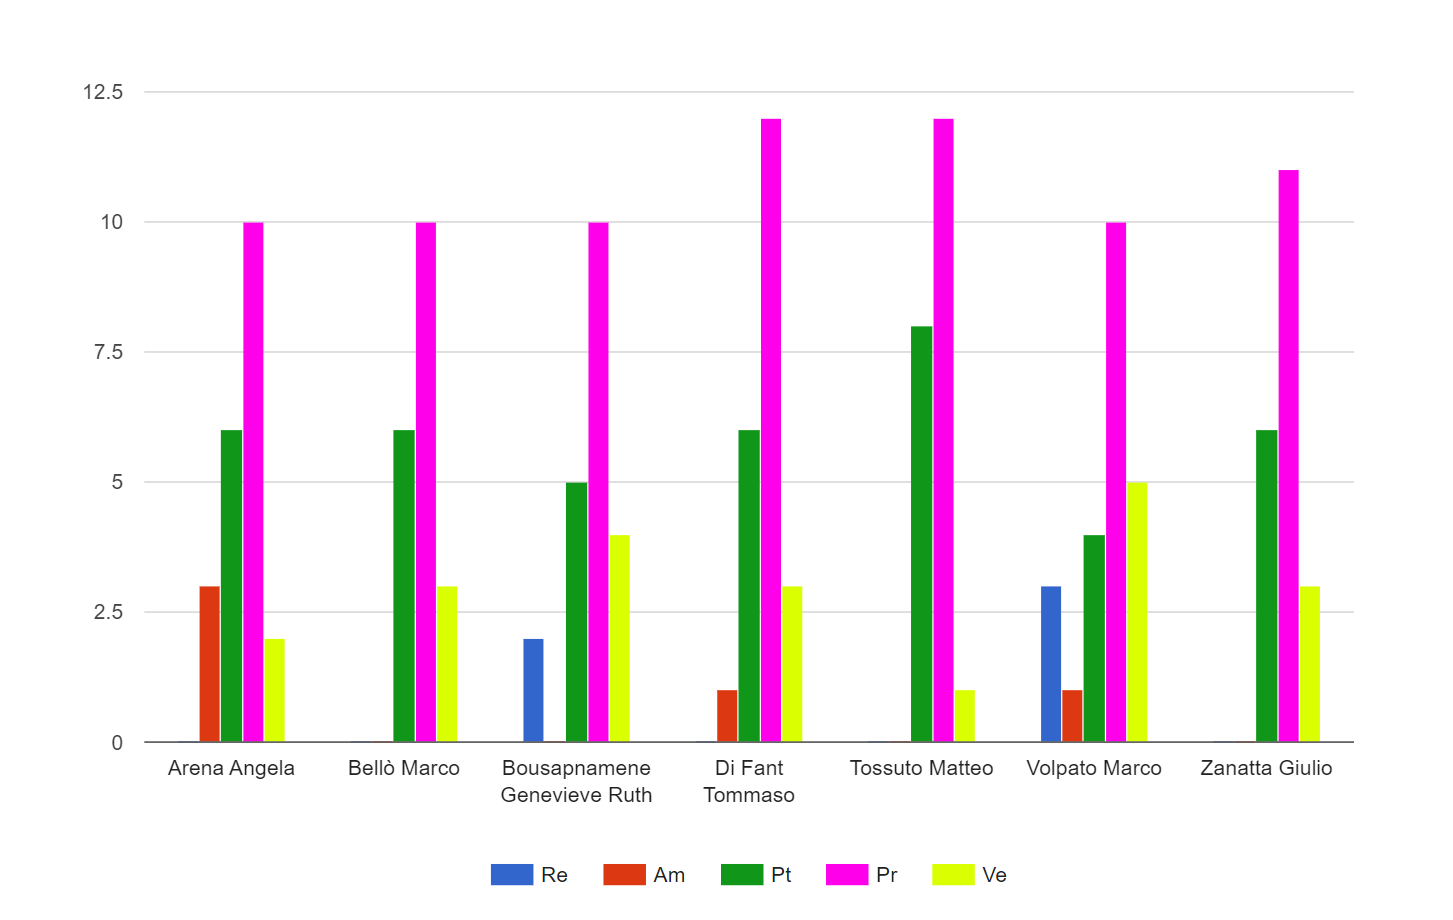
\includegraphics[width=15cm]{sezioni/images/quinto.png}
        \centering
        \caption{Quinto incremento - Istogramma suddivisone ore per ruolo}
     \end{figure}
    }

    \subsubsection{Prospetto Economico}
    {
        \setlength{\freewidth}{\dimexpr\textwidth-30\tabcolsep}
        \renewcommand{\arraystretch}{1.0}
        \setlength{\aboverulesep}{0pt}
        \setlength{\belowrulesep}{0pt}
        \rowcolors{2}{Arancione!10}{white}
        \begin{longtable}{C{.4\freewidth} C{.2\freewidth} C{.2\freewidth} C{.2\freewidth} C{.2\freewidth} C{.2\freewidth} C{.2\freewidth} C{.2\freewidth} C{.2\freewidth}}
          \toprule
        \rowcolor{Arancione}
        \textcolor{white}{\textbf{Ruolo}}&
        \textcolor{white}{\textbf{Ore}}&
        \textcolor{white}{\textbf{Costo}}\\
        \toprule
        \endhead
            
        Responsabile  & 5 & \euro150\\
        Amministratore  & 7 & \euro140 \\
        Analista &- & -\\
        Progettista &41 &\euro1025\\
        Programmatore &75 & \euro1125\\
        Verificatore &21 &\euro315\\
        Totale&148&\euro2755\\
        \bottomrule
      \\
      \rowcolor{white}
        \caption{Quinto incremento - Costo per ruolo}

        \end{longtable}
        \begin{figure}[H]
          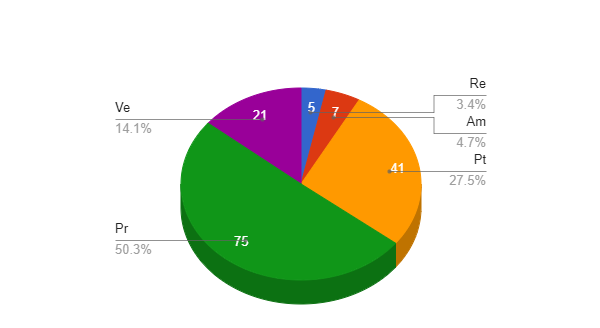
\includegraphics[width=15cm]{sezioni/images/quintoT.png}
          \centering
          \caption{Quinto incremento - Grafico a torta costo per ruolo}
       \end{figure}
    }
    }

    \subsection{Sesto incremento} 
    {
    \subsubsection{Prospetto orario}
    {
    Il gruppo per il sesto incremento si impegna a rispettare la suddivisione oraria dei ruoli come riportato in tabella:
      \setlength{\freewidth}{\dimexpr\textwidth-30\tabcolsep}
      \renewcommand{\arraystretch}{1.0}
      \setlength{\aboverulesep}{0pt}
      \setlength{\belowrulesep}{0pt}
      \rowcolors{2}{Arancione!10}{white}
      \begin{longtable}{C{.4\freewidth} C{.1\freewidth} C{.1\freewidth} C{.1\freewidth} C{.1\freewidth} C{.1\freewidth} C{.1\freewidth} C{.1\freewidth} C{.1\freewidth}}
      \toprule
      \rowcolor{Arancione}
      \textcolor{white}{\textbf{Componente}}&
      \textcolor{white}{\textbf{Re}}&
      \textcolor{white}{\textbf{Am}}&
      \textcolor{white}{\textbf{An}}&
      \textcolor{white}{\textbf{Pt}}&
      \textcolor{white}{\textbf{Pr}}&
      \textcolor{white}{\textbf{Ve}}&
      \textcolor{white}{\textbf{Ore}}\\
      \toprule
      \endhead

      Arena Angela & 4 & - & -  & 1 & 3 & 4 & 12 \\      
      Bellò Marco & 3 & - & - & 2 & 6 & 2 & 13 \\      
      Bousapnamene & - & - & - & 3 & 7 & 2 & 13 \\      
      Di Fant Tommaso & - & - & - & 1 & 8 & 4 & 13 \\      
      Tossuto Matteo & - & - & - & 3 & 8 & 1 & 12 \\      
      Volpato Marco & - & - & - & 2 & 9 & 3 & 14 \\      
      Zanatta Giulio & - & - & - & 2 & 8 & 2 & 12 \\      
      Totali & 7 & - & - & 14 & 49 & 18 & 89 \\
      \bottomrule
      \rowcolor{white}
      \\
      \caption{Sesto incremento - Suddivisone ore per ruolo}

      \end{longtable} 

      \begin{figure}[H]
        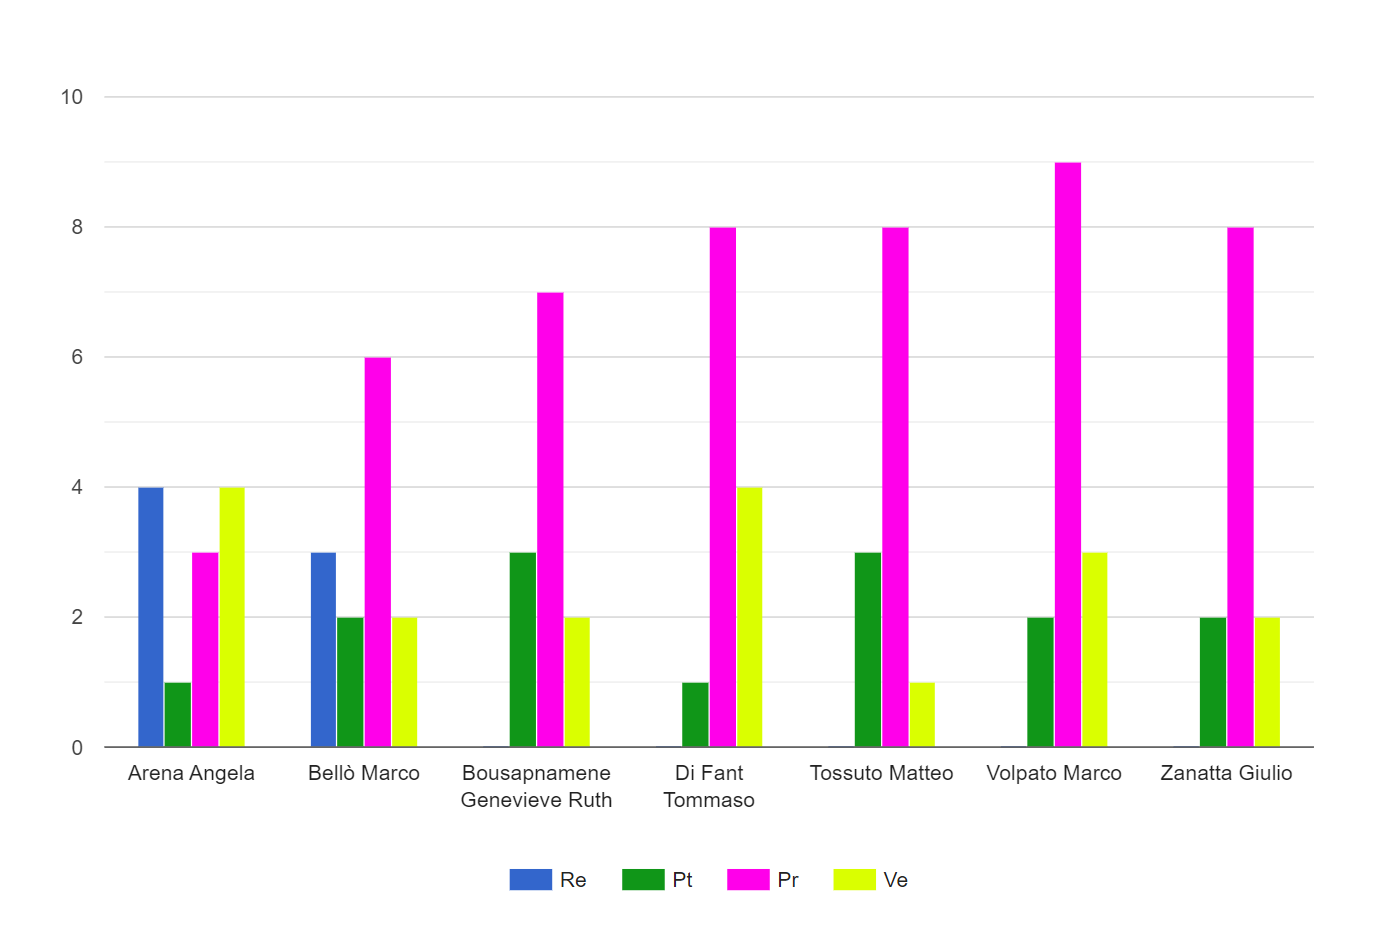
\includegraphics[width=15cm]{sezioni/images/sesto.png}
        \centering
        \caption{Sesto incremento - Istogramma suddivisone ore per ruolo}
     \end{figure}
    }

    \subsubsection{Prospetto Economico}
    {
        \setlength{\freewidth}{\dimexpr\textwidth-30\tabcolsep}
        \renewcommand{\arraystretch}{1.0}
        \setlength{\aboverulesep}{0pt}
        \setlength{\belowrulesep}{0pt}
        \rowcolors{2}{Arancione!10}{white}
        \begin{longtable}{C{.4\freewidth} C{.2\freewidth} C{.2\freewidth} C{.2\freewidth} C{.2\freewidth} C{.2\freewidth} C{.2\freewidth} C{.2\freewidth} C{.2\freewidth}}
          \toprule
        \rowcolor{Arancione}
        \textcolor{white}{\textbf{Ruolo}}&
        \textcolor{white}{\textbf{Ore}}&
        \textcolor{white}{\textbf{Costo}}\\
        \toprule
        \endhead
            
        Responsabile  & 7 & \euro210\\
        Amministratore  & - & - \\
        Analista &- & -\\
        Progettista &14 &\euro350\\
        Programmatore &49 & \euro735\\
        Verificatore &18 &\euro270\\
        Totale&89&\euro1565\\
        \bottomrule
      \\
      \rowcolor{white}
        \caption{Sesto incremento - Costo per ruolo}

        \end{longtable}
        \begin{figure}[H]
          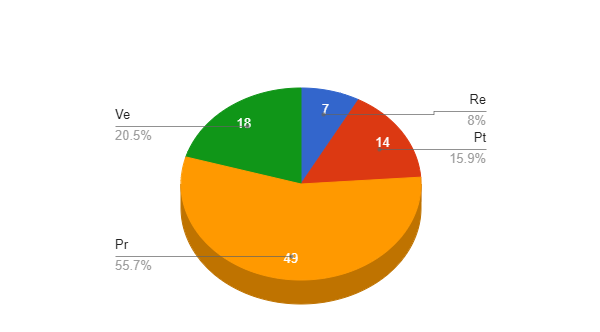
\includegraphics[width=15cm]{sezioni/images/sestoT.png}
          \centering
          \caption{Sesto incremento - Grafico a torta costo per ruolo}
       \end{figure}
    }
    }

    \subsection{Settimo incremento} 
    {
    \subsubsection{Prospetto orario}
    {
    Il gruppo per il settimo incremento si impegna a rispettare la suddivisione oraria dei ruoli come riportato in tabella:
      \setlength{\freewidth}{\dimexpr\textwidth-30\tabcolsep}
      \renewcommand{\arraystretch}{1.0}
      \setlength{\aboverulesep}{0pt}
      \setlength{\belowrulesep}{0pt}
      \rowcolors{2}{Arancione!10}{white}
      \begin{longtable}{C{.4\freewidth} C{.1\freewidth} C{.1\freewidth} C{.1\freewidth} C{.1\freewidth} C{.1\freewidth} C{.1\freewidth} C{.1\freewidth} C{.1\freewidth}}
      \toprule
      \rowcolor{Arancione}
      \textcolor{white}{\textbf{Componente}}&
      \textcolor{white}{\textbf{Re}}&
      \textcolor{white}{\textbf{Am}}&
      \textcolor{white}{\textbf{An}}&
      \textcolor{white}{\textbf{Pt}}&
      \textcolor{white}{\textbf{Pr}}&
      \textcolor{white}{\textbf{Ve}}&
      \textcolor{white}{\textbf{Ore}}\\
      \toprule
      \endhead

      Arena Angela & - & 1 & -  & 2 & 3 & 4 & 13 \\      
      Bellò Marco & - & 2 & - & 2 & 3 & 5 & 12 \\      
      Bousapnamene & - & 2 & - & 1 & 4 & 4 & 11 \\      
      Di Fant Tommaso & 3 & 2 & - & 3 & 2 & 2 & 12 \\      
      Tossuto Matteo & 5 & 1 & - & 1 & 1 & 3 & 12 \\      
      Volpato Marco & - & - & - & 5 & 3 & 4 & 12 \\      
      Zanatta Giulio & - & 2 & - & 3 & 3 & 5 & 12 \\      
      Totali & 8 & 10 & - & 18 & 20 & 27 & 84 \\
      \bottomrule 
       \rowcolor{white}
      \\
      \caption{\centering{Settimo incremento - Suddivisone ore per ruolo}}

      \end{longtable} 

      \begin{figure}[H]
        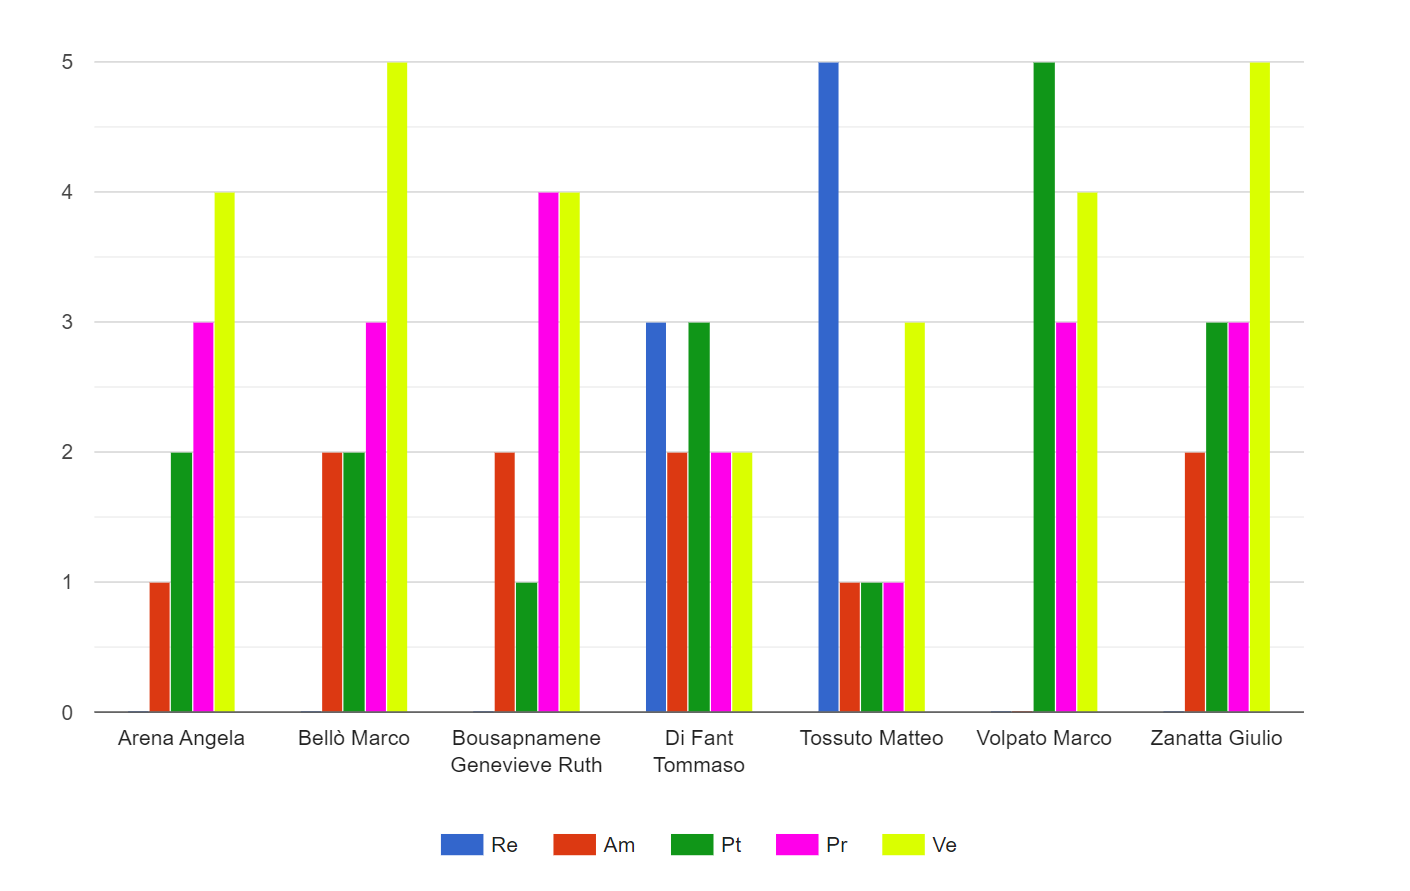
\includegraphics[width=15cm]{sezioni/images/settimo.png}
        \centering
        \caption{Settimo incremento - Istogramma suddivisone ore per ruolo}
     \end{figure}
    }

    \subsubsection{Prospetto Economico}
    {
        \setlength{\freewidth}{\dimexpr\textwidth-30\tabcolsep}
        \renewcommand{\arraystretch}{1.0}
        \setlength{\aboverulesep}{0pt}
        \setlength{\belowrulesep}{0pt}
        \rowcolors{2}{Arancione!10}{white}
        \begin{longtable}{C{.4\freewidth} C{.2\freewidth} C{.2\freewidth} C{.2\freewidth} C{.2\freewidth} C{.2\freewidth} C{.2\freewidth} C{.2\freewidth} C{.2\freewidth}}
          \toprule
        \rowcolor{Arancione}
        \textcolor{white}{\textbf{Ruolo}}&
        \textcolor{white}{\textbf{Ore}}&
        \textcolor{white}{\textbf{Costo}}\\
        \toprule
        \endhead
            
        Responsabile  & 8 & \euro240\\
        Amministratore  & 10 & \euro200 \\
        Analista &- & -\\
        Progettista &18 &\euro450\\
        Programmatore &20 & \euro300\\
        Verificatore &27 &\euro405\\
        Totale&84&\euro1595\\
        \bottomrule
      \\
      \rowcolor{white}
        \caption{Settimo incremento - Costo per ruolo} 

        \end{longtable}

        \begin{figure}[H]
          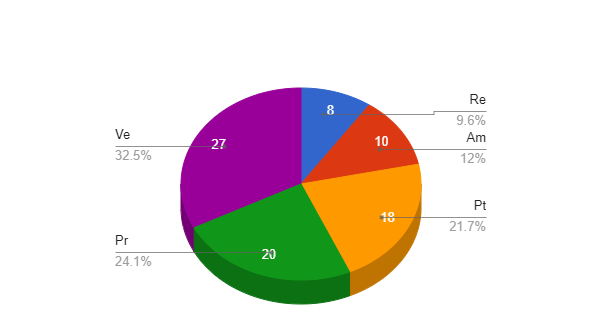
\includegraphics[width=15cm]{sezioni/images/settimoT.png}
          \centering
          \caption{Settimo incremento - Grafico a torta costo per ruolo}
       \end{figure}
    }
    }

    \subsection{Ottavo incremento} 
    {
    \subsubsection{Prospetto orario}
    {
    Il gruppo per il ottavo incremento si impegna a rispettare la suddivisione oraria dei ruoli come riportato in tabella:
      \setlength{\freewidth}{\dimexpr\textwidth-30\tabcolsep}
      \renewcommand{\arraystretch}{1.0}
      \setlength{\aboverulesep}{0pt}
      \setlength{\belowrulesep}{0pt}
      \rowcolors{2}{Arancione!10}{white}
      \begin{longtable}{C{.4\freewidth} C{.1\freewidth} C{.1\freewidth} C{.1\freewidth} C{.1\freewidth} C{.1\freewidth} C{.1\freewidth} C{.1\freewidth} C{.1\freewidth}}
      \toprule
      \rowcolor{Arancione}
      \textcolor{white}{\textbf{Componente}}&
      \textcolor{white}{\textbf{Re}}&
      \textcolor{white}{\textbf{Am}}&
      \textcolor{white}{\textbf{An}}&
      \textcolor{white}{\textbf{Pt}}&
      \textcolor{white}{\textbf{Pr}}&
      \textcolor{white}{\textbf{Ve}}&
      \textcolor{white}{\textbf{Ore}}\\
      \toprule
      \endhead

      Arena Angela & - & 1 & -  & - & 1 & 5 & 7 \\      
      Bellò Marco & - & 2 & - & - & 1 & 4 & 7 \\      
      Bousapnamene & - & 1 & - & - & 1 & 4 & 6 \\      
      Di Fant Tommaso & - & - & - & - & 1 & 5 & 6 \\      
      Tossuto Matteo & - & 2 & - & - & 1 & 4 & 7 \\      
      Volpato Marco & - & 2 & - & - & 1 & 3 & 6 \\      
      Zanatta Giulio & 3 & - & - & - & 1 & 3 & 7 \\      
      Totali & 3 & 8 & - & - & 7 & 28 & 46 \\
      \bottomrule  
       \rowcolor{white}
      \\
      \caption{\centering{Ottavo incremento - Suddivisione ore per ruolo}}

      \end{longtable} 

      \begin{figure}[H]
        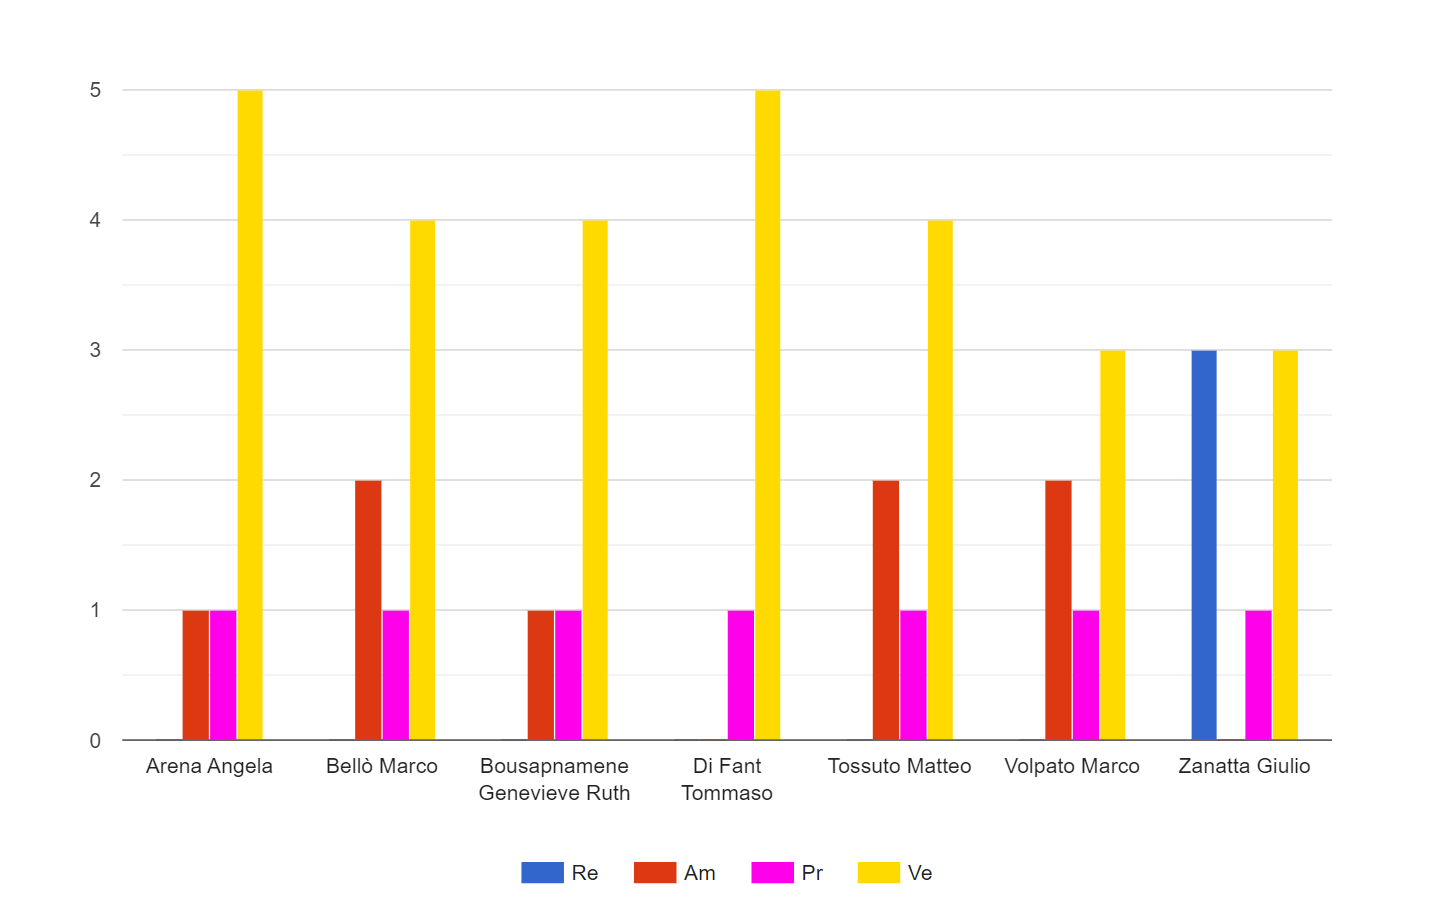
\includegraphics[width=15cm]{sezioni/images/ottavo.png}
        \centering
        \caption{Ottavo incremento - Istogramma suddivisione ore per ruolo}
     \end{figure}
    }

    \subsubsection{Prospetto Economico}
    {
        \setlength{\freewidth}{\dimexpr\textwidth-30\tabcolsep}
        \renewcommand{\arraystretch}{1.0}
        \setlength{\aboverulesep}{0pt}
        \setlength{\belowrulesep}{0pt}
        \rowcolors{2}{Arancione!10}{white}
        \begin{longtable}{C{.4\freewidth} C{.2\freewidth} C{.2\freewidth} C{.2\freewidth} C{.2\freewidth} C{.2\freewidth} C{.2\freewidth} C{.2\freewidth} C{.2\freewidth}}
          \toprule
        \rowcolor{Arancione}
        \textcolor{white}{\textbf{Ruolo}}&
        \textcolor{white}{\textbf{Ore}}&
        \textcolor{white}{\textbf{Costo}}\\
        \toprule
        \endhead
            
        Responsabile  & 3 & \euro90\\
        Amministratore  & 8 & \euro160 \\
        Analista &- & -\\
        Progettista &- &-\\
        Programmatore &7 & \euro105\\
        Verificatore &28 &\euro420\\
        Totale&46&\euro775\\
        \bottomrule
      \\
      \rowcolor{white}
        \caption{Ottavo incremento - Costo per ruolo}
        \end{longtable}

        \begin{figure}[H]
          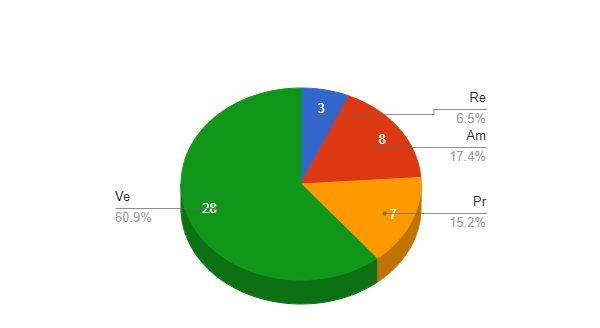
\includegraphics[width=15cm]{sezioni/images/ottavoT.png}
          \centering
          \caption{Ottavo incremento - Grafico a torta costo per ruolo}
       \end{figure}
    }

    }


